\begin{frame}
	\textbf{Wage Equations}
	\begin{align*}
	\ln W_1 & = \ln \pi_1 + \mu_1 + U_1 \\
	\ln W_2 & = \ln \pi_2 + \mu_2 + U_2, \\
	\end{align*}
	where $U_i = \ln S_i - \mu_i$.
\end{frame}
%-------------------------------------------------------------------------------
%-------------------------------------------------------------------------------
\begin{frame}
	\textbf{Sorting}
	\begin{align*}
	E[\ln S_1 \mid \ln W_1 > \ln W_2] & = \mu_1 + \frac{\sigma_{11} - \sigma_{12}}{\sigma^*} \lambda(-c_1) \\
	E[\ln S_2 \mid \ln W_2 > \ln W_1] & = \mu_2 + \frac{\sigma_{22} - \sigma_{12}}{\sigma^*} \lambda(-c_2)
	\end{align*}
	We know the following:
	\begin{align*}
	\sigma^* & = (\sigma_{11} - \sigma_{12}) +  (\sigma_{22} - \sigma_{12}) > 0 \\
	\lambda &> 0
	\end{align*}
	\begin{itemize}\setlength\itemsep{1em}
		\item There must be positive selection into one of the occupations and there can be positive selection into both.
	\end{itemize}	
\end{frame}
%-------------------------------------------------------------------------------
%-------------------------------------------------------------------------------
\begin{frame}
	\begin{figure}[htp]\centering
		\caption{Marginal Distributions of Skills}\label{Marginal Distributions of Skills}\scalebox{0.35}{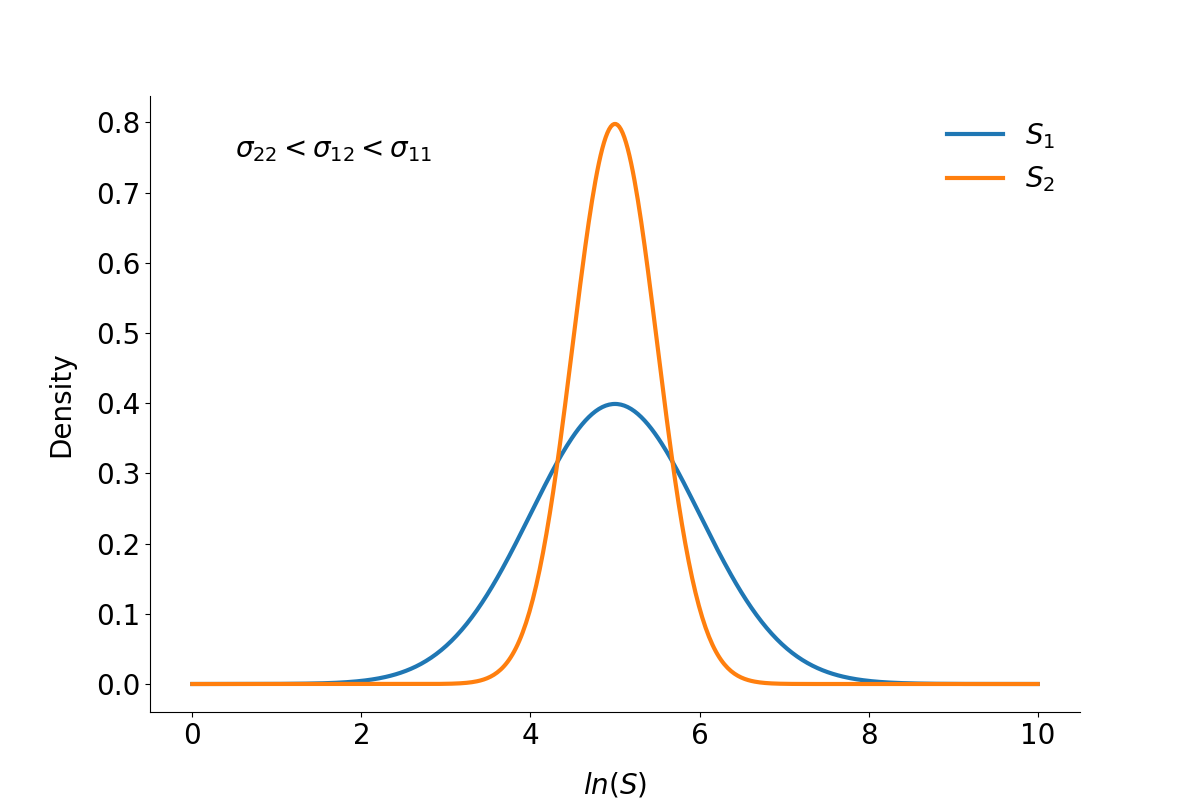
\includegraphics{fig-distribution-skills-latent-marginal-two}}
	\end{figure}
\end{frame}
%-------------------------------------------------------------------------------
%-------------------------------------------------------------------------------
\begin{frame}
	\textbf{What do we know?}
	\begin{itemize}\setlength\itemsep{1em}
		\item There is positive selection in Sector 2, because there cannot be negative selection in both and $\sigma_{22} > \sigma_{11}$.
	\end{itemize}\medskip
	\textbf{How about Sector 1?}
	\begin{itemize}\setlength\itemsep{1em}
		\item If $\sigma_{12} < 0$, then there is also positive selection in Sector 1.
		\item If $\rho_{12} = 1$, then there is negative selection into Sector 1 as $\sigma_{12} > \sigma_{11}$
	\end{itemize}
\end{frame}
%-------------------------------------------------------------------------------
%-------------------------------------------------------------------------------
\begin{frame}
	We gain further insights into the effect of self-selection on the distribution of earnings for workers in sector 1 by looking at the  distribution of $\ln S_1$  conditional on $\ln S_2$.	
	\begin{align*}
	\ln S_1 \mid \ln S_2 \sim \N (\mu, \sigma),
	\end{align*}
	where
	\begin{align*}
	\mu = \mu_1 + \frac{\sigma_{12}}{\sigma_{22}} \Bigg(\ln S_2 - \mu_2\Bigg) \quad\text{and}\quad
	\sigma = \sigma_{11} \left(1 - \left(\frac{\sigma_{12}}{\sigma_1 \sigma_2}\right)^2\right)
	\end{align*}	
\end{frame}